\documentclass[12pt]{article}
\usepackage[utf8]{inputenc}
\usepackage[T1]{fontenc}

\usepackage{bm}							% bold math symbols
\usepackage{amsmath}					% equation formatting
\usepackage{amssymb}					% equation symbols
\usepackage{mathtools}					% amsmath extension, symbols
\usepackage{siunitx}					% SI units package
\usepackage{caption}					% extended caption functionality
\usepackage{subcaption}					% provides subcaptions
\usepackage{graphicx}					% images
\usepackage{xcolor}						% driver-independent colors
\usepackage{wrapfig}					% figure wrapping
\usepackage{tikz}						% portable graphics format creator
\usetikzlibrary{decorations.pathreplacing}

\usepackage[margin=1in]{geometry}		% document layout package

\usepackage[notes,backend=biber]{biblatex-chicago} % citation styling
\usepackage[english]{babel}				% language package
\usepackage[autostyle=true]{csquotes}	% extended quotation functionality
\usepackage{hyperref}					% hypertext support

\usepackage{setspace}					% easy text spacing
\usepackage{newtxtext,newtxmath} 		% times new roman, more up to date

% Standard ihat and jhat are not implemented by default.
% This provides the ihat and jhat without the dot at the top.
% Is basic implementation, does not work with mathptmx
%\newcommand{\ihat}{\mathbf {\hat \imath}}
%\newcommand{\jhat}{\mathbf {\hat \jmath}}

% Declare bibliography as the 'references.bib' file
\bibliography{references}

% Set doublespacing
\doublespacing
%\renewcommand{\baselinestretch}{1.5}

% Custom text formatting
\setlength{\parindent}{0pt}
\setlength{\parskip}{1em}

% Renaming the 'Contents' field to 'Table of Contents'
\addto\captionsenglish{ % required by babel
	\renewcommand{\contentsname}{Table of Contents}
}

% implementation of a unit vector as given by 'egreg' from tex.stackexchange.com 
% https://tex.stackexchange.com/questions/188775/how-to-type-a-particular-kind-of-unit-vector
\newcommand{\uveci}{{\bm{\hat{\textnormal{\bfseries\i}}}}}
\newcommand{\uvecj}{{\bm{\hat{\textnormal{\bfseries\j}}}}}
\DeclareRobustCommand{\uvec}[1]{{%
		\ifcat\relax\noexpand#1%
		% it should be a Greek letter
		\bm{\hat{#1}}%
		\else
		\ifcsname uvec#1\endcsname
		\csname uvec#1\endcsname
		\else
		\bm{\hat{\mathbf{#1}}}% This really is the only important thing
		\fi
		\fi
}}

\newcommand{\bvec}[1]{\bm{\mathbf{#1}}}

\captionsetup[figure]{font=small,justification=centering}

\allowdisplaybreaks

\begin{document}
	\begin{titlepage}
	\begin{center}
		\vspace*{\fill}
		
		The Mathematics behind Lagrange Points
		
		\vspace*{1.0cm}
		Word Count: \#\#\#\#
		
		\vfill
		
		Julian Joaquin\\
		Mathematics Internal Assessment\\
		Professor\\
		Date
		
		\vspace*{\fill}
		
	\end{center}
\end{titlepage}
	
	\tableofcontents
	
	\newpage
	
	\section{Introduction}
	
	With the deployment of the James Webb Space Telescope, many people are excited to see what discoveries it will uncover about the Universe.
	Its development has involved bleeding edge technology and engineering innovations, most of which have the intent to keep the telescope cool. % CITATION NEEDED!
	One aspect of the JWST that is not well understood by most people are Lagrange points and how a satellite can be positioned in one of these points.
	High school physics teaches us that satellites can orbit around stars and planets because of gravity.
	Yet, when the JWST will orbit around Lagrange point 2, it appears as if the telescope is orbiting around nothing!
	How is this possible?
	
	This investigation aims to locate the collinear Sun-Earth Lagrange points and attempt to model the orbit of a satellite around a Lagrange point using IB level mathematics.
	Identifying the locations of the Lagrange points will involve an understanding of algebra and Newtonian mechanics.
	The derivation of the halo orbits around the Lagrange points will be more complex, requiring vectors, calculus, and a bit of linear algebra.
	
	\section{Finding the Lagrange Points}
	
	We will be determining the collinear Lagrange points from a rotating frame of reference relative to a circular orbit of Earth.
	This simplifies the solution to a single dimension which bisects the Sun and Earth. % ELABORATE
	
	\vspace*{0.5cm}
	\begin{figure}[!h]
		\centering
		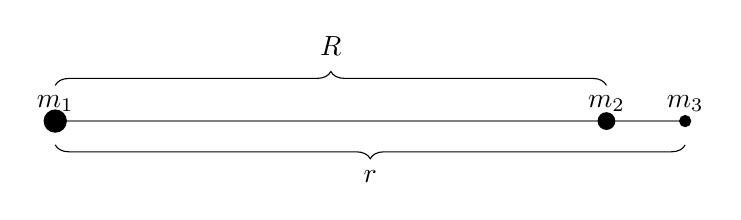
\begin{tikzpicture}
			\draw[gray,thick] (-4,0) -- (4,0);
			\filldraw (-4,0) circle (4pt) node[anchor=south]{$m_1$};
			\filldraw (3,0) circle (3pt) node[anchor=south]{$m_2$};
			\filldraw (4,0) circle (2pt) node[anchor=south]{$m_3$};
			\draw[decorate,decoration={brace,amplitude=5pt,raise=3ex}] (-4,0) -- (3,0) node[midway,yshift=27pt]{$R$};
			\draw[decorate,decoration={brace,mirror,amplitude=5pt,raise=2ex}] (-4,0) -- (4,0) node[midway,yshift=-2em]{$r$};
		\end{tikzpicture}
		\vspace*{0.25cm}
		\caption{Simple diagram of the Sun-Earth system.}
		\label{fig:collinear-coords}
	\end{figure}

	\textit{R} will be the distance between the Sun and Earth, while \textit{r} will be the distance from the main body to the Lagrange point. 
	The masses of the Sun, Earth, and a point located at the Lagrange point are denoted by $m_1$, $m_2$, and $m_3$, respectively.
	For the sake of maintaining direction, bodies positioned to the right will have a positive distance, and vice versa.

	It is important to understand what factors are at play when dealing with Lagrange points.
	What will be most important is Newton's Law of Gravitation,
	\begin{equation}
		F = \frac{Gm_1m_2}{r^2}
	\end{equation}
	where \textit{F} is the force exerted between two bodies of mass, \textit{G} is the gravitational constant, m is the mass of a body, and \textit{r} is the distance between the two bodies.
	%The sum of forces acting on our fictional object $m_3$ due to gravity is then
	%\begin{equation}
	%	F = -\frac{Gm_1m_3}{r^3} - \frac{Gm_2m_3}{(r-R)^3}
	%\end{equation}
	We must also consider the centrifugal and Coriolis forces acted on the object at the Lagrange point.
	We can rule out the Coriolis force, since the collinear Lagrange points will not be moving in our rotating frame of reference.
	As for centrifugal force, it will be proportional to the centripetal force,
	\begin{equation}
		F = m\omega^2r
	\end{equation}
	where $\omega$ is the angular velocity of the object. Understanding that angular velocity can be defined as
	\begin{equation}
		\omega = \frac{2\pi}{T}
	\end{equation}
	and the period of a circular orbit, from Kepler's third law, as
	\begin{equation}
		T = 2\pi\sqrt{\frac{R^3}{G(m_1+m_2)}} % NOTE: this may require citation.
	\end{equation}
 	the equation for angular velocity simplifies to
 	\begin{equation}
 		\omega^2 = \frac{G(m_1+m_2)}{R^3} \text{.} % NOTE: Gravitational Parameter is the sum of the two major masses. Citation^^?
 	\end{equation} % You should add details as to why we are evaluating the radial acceleration. THERE IS A DISCEPENCY IN THE ALGREBRA!
	Therefore, the sum of forces acting on an object at a Lagrange point is
	\begin{equation}
		F = m_3a = -\frac{Gm_1m_3}{r^2} - \frac{Gm_2m_3}{(r - R)^2} + \frac{G(m_1+m_2)}{R^3}rm_3 \text{.}
	\end{equation}
	Solving for a radial acceleration of 0, we get the formula
	\begin{equation}
		0 = -\frac{Gm_1}{r^2} - \frac{Gm_2}{(r - R)^2} + \frac{G(m_1+m_2)}{R^3}r \text{.}
	\end{equation}
	Most of the variables are known constants, with \textit{r} being the only unknown value which represents the distance of the Lagrange point from $m_1$.
	It is worth noting that, with respect to direction, $r^2$ and $(r-R)^2$ will only reflect acceleration in the negative direction and will not be sufficient to tell us where L1 and L3 are.
	To remedy this, the formula is rewritten as such to preserve the sign of $r$:
	\begin{equation}
		0 = -\frac{Gm_1}{r|r|} - \frac{Gm_2}{(r - R)|r - R|} + \frac{G(m_1+m_2)}{R^3}r \text{.}
	\end{equation}
	%The sign of each term in the equation is important to represent which direction acceleration is being applied.
	%If $m_3$ were positioned between $m_1$ and $m_2$, for example, than the term $-\frac{Gm_2}{(r-R^2)}$ should be positive to show that the acceleration caused by the gravity of $m_2$ is in the outward direction.
	%However, for each of the gravity terms in our equation, $r^2$ and $(r-R)^2$ will always be positive regardless ...
	Further simplification of the formula results in a rational function that is almost impossible to solve by hand, in part because the formula would involve significantly large values due to the constants used.
	Instead, the roots of the formula are solved for computationally.
	\begin{figure}[h!]
		\centering
		\captionsetup[subfigure]{justification=centering}
		\begin{subfigure}[b]{0.4\textwidth}
			\centering
			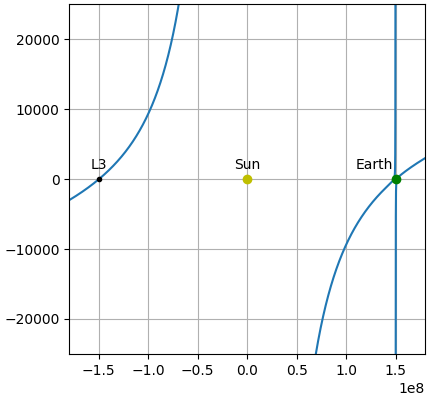
\includegraphics[scale=0.6]{r-accel-figure-1.png}
			\caption{\footnotesize Radial Acceleration between the Sun and Earth.}
			\label{fig:radial-accel-system}
		\end{subfigure}
		\hspace*{1cm}
		\begin{subfigure}[b]{0.4\textwidth}
			\centering
			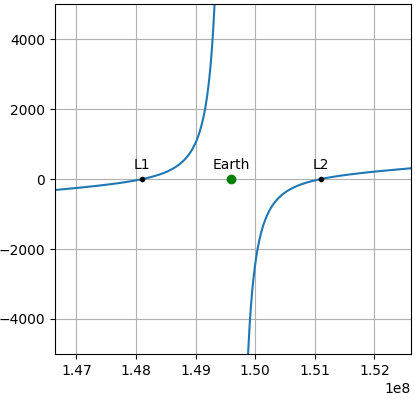
\includegraphics[scale=0.6]{r-accel-figure-2.png}
			\caption{\footnotesize Radial acceleration around the Earth.\vspace*{1.16em}}
			\label{fig:radial-accel-earth}
		\end{subfigure}
		\label{fig:radial-accel}
		\caption{Net acceleration of the Sun-Earth system. Graphs are created using \texttt{matplotlib}.}
	\end{figure} % this figure can benefit from an explanation

	%\begin{figure}[h!]
	%	\centering
	%	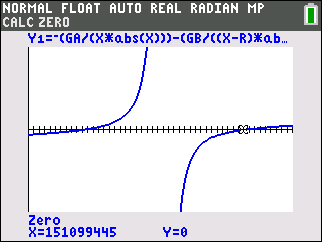
\includegraphics[scale=0.7]{accel-root.png}
	%	\caption{Solution for L2 using a GDC.}
	%	\label{fig:radial-l2}
	%\end{figure}
	Relative to the distance from the sun, the locations of the Lagrange points are as follows.
	\begin{table}[h!]
		\centering
		\label{tab:lagrange-points}
		\caption{Distance of the collinear Lagrange points from the Sun}
		\vspace*{0.3cm}
		\begin{tabular}{|r|l|}
			\hline
			L1 & $1.481\times10^8 \si{\kilo\metre}$ \\
			\hline
			L2 & $1.511\times10^8 \si{\kilo\metre}$ \\
			\hline
			L3 & $-1.496\times10^8 \si{\kilo\metre}$ \\
			\hline
		\end{tabular}
	\end{table}
	
	\section{Setup Scenarios for Equations of Motion}
	
	As stated in the introduction, finding out the motion of a satellite around a Lagrange point will be incredibly difficult.
	To prepare for this, let us take a step back and tackle these two scenarios.
	
	\subsection{Simple Linear Differential Equations} \label{sec:ode}
	
	For our first scenario, let us imagine that, for some function $n$ with respect to $t$,
	\begin{equation}\label{eqn:lde1}
		\frac{dn}{dt} = 4n
	\end{equation}
	In words, the rate of change of the function is equal to itself multiplied by four. Let us say we wanted to find what function $n$ is.
	While it is not as simple to just integrate this equation, we know that $e^x$ is its own derivative.
	We also know that, because of the chain rule, $[e^{kt}]' = ke^{kt}$.
	If we substitute $n$ for $e^{kx}$ and let $k = 4$, then equation \eqref{eqn:lde1} is true.
	Therefore, we can state the following theorem; for some equation
	\begin{equation}\label{eqn:theory1}
		\frac{dn}{dt} = kn\ \text{,} \quad n = ce^{kt}
	\end{equation}
	where $c$ is some initial constant that cannot be expressed from integrating the derivative.
	We can verify that this theorem is correct using some algebra and integration.
	\begin{align*}
		\frac{dn}{dt} &= kn \\
		\frac{1}{n}\, dn &= k\, dt \\
		\int \frac{1}{n}\, dn &= \int k\, dt \\
		\ln n + C &= kt + D \\
		\ln n &= kt + (D - C) \\
		n &= e^{kt} \cdot e^{D - C} \hspace*{3em}
	\end{align*}
	This will become handy for equations that are only defined by their derivative.
	
	\subsection{Systems of Linear Differential Equations} \label{sec:ode-sys}
	
	The second scenario builds off the first, and involves equations that are defined by each other.
	Consider the following system of equations with functions $x$ and $y$ in terms of $t$:
	\begin{align}
		\frac{dx}{dt} &= 4x - 2y \quad &x(0) = 4 \\
		\frac{dy}{dt} &= 3x - y \quad &y(0) = 2
	\end{align}
	Here, the rate of change of $x$ is defined in terms of both $x$ and $y$, and same goes for the rate of change of $y$.
	Because these two equations are intertwined, initially it seems impossible to define both $x$ and $y$ as separate from each other.
	However, remembering our previous theorem, Equation \eqref{eqn:theory1}, we can predict that both functions will look something like this:
	\begin{align}
		x(t) = c_1e^{r_1t} + c_2e^{r_1t} \label{eqn:x-t-general}\\
		y(t) = c_1e^{r_2t} + c_2e^{r_2t} \label{eqn:y-t-general}
	\end{align}
	Also from Equation \eqref{eqn:theory1}, let us imagine that it is possible to state the rate of change as function of itself multiplied by a constant, $k$.
	\begin{align}
		\frac{dx}{dt} &= kx = 4x - 2y \label{eqn:kx-sys}\\
		\frac{dy}{dt} &= ky = 3x - y \label{eqn:ky-sys}
	\end{align}
	Forgetting the fact that we are involving derivatives for a moment, we can try solving for $k$ by solving this linear system though substitution.
	\begin{align}
		4x - 2y &= kx \nonumber \\
		(4 - k)x &= 2y \nonumber \\
		\frac{(4 - k)x}{2} &= y \nonumber \\
		3x - y &=ky \nonumber \\
		3x &= (k + 1)y \nonumber \\
		3x &= (k + 1)\frac{(4 - k)x}{2} \nonumber \\
		3\times2 &= (k + 1)(4 - k) \nonumber \\
		0 &= (1 + k)(4 - k) - 3\times2 \label{eqn:chr-polynomial-ex}
	\end{align}
	By now, we can deduce that there will be two possible values for $k$.
	Continuing the solution,
	\begin{align}
		0 &= -k^2 - 3k + 2 \nonumber \\
		0 &= (k - 1)(k - 2)
	\end{align}
	Here, the solutions are $k_1 = 1$ and $k_2 = 2$.
	We don't know exactly what these values \textit{mean}, other than they correspond to $x$ and $y$, respectively.
	Let us see what happens when we plug them into our linear system.
	For $k_1$:
	\begin{equation}
		\left. \begin{array}{l}
			(1)x = 4x - 2y \\
			(1)y = 3x - y
		\end{array} \right \}
		\implies 0 = 3x - 2y \implies 2y = 3x
	\end{equation}
	This gives us a relationship of $x$ and $y$ where, when $k = 1$, there is a 
	$2 : 3$ ratio between $x$ and $y$.
	This is significant because, for some specific values of $x$, $y$, and $k$, our system of linear equations \textit{converge} in a manner that essentially defines them as the same equation.
	This is easier to understand when graphed.
	\begin{figure}[h!]
		\centering
		\captionsetup[subfigure]{justification=centering}
		\begin{subfigure}[b]{0.4\textwidth}
			\centering
			\begin{tikzpicture}
				\draw (-3,0) -- (3,0) node[right] {$x$};
				\draw (0,-3) -- (0,3) node[above] {$y$};
				\draw[thick,green] (-1.5, -3) -- (1.5,3);
				\draw[thick,dashed,red] (-1,-3) -- (1,3);
				\node at (1,-1) [right,align=right] {$\textcolor{green}{4x - 2x = kx}$ \\
				$\textcolor{red}{3x - y = ky}$ \\
				$\textcolor{black}{k = 0}$};
			\end{tikzpicture}
			\caption{\small Linear system with $k = 0$.}
			\label{fig:sample-eigens0}
		\end{subfigure}
		\qquad
		\begin{subfigure}[b]{0.4\textwidth}
			\centering
			\begin{tikzpicture}
				\draw (-3,0) -- (3,0) node[right] {$x$};
				\draw (0,-3) -- (0,3) node[above] {$y$};
				\draw[thick,green] (-2, -3) -- (2,3);
				\draw[thick,dashed,red] (-2,-3) -- (2,3);
				\filldraw[black] (1,1.5) circle (1.25pt) node[anchor=west] {$\textcolor{black}{(2,3)}$};
				\node at (1,-1) [right,align=right] {$\textcolor{green}{4x - 2x = kx}$ \\
				$\textcolor{red}{3x - y = ky}$ \\
				$\textcolor{black}{k = 1}$};
			\end{tikzpicture}
		\caption{\small Linear system with $k = 1$.}
		\label{fig:sample-eigens1}
		\end{subfigure}
		\caption{The linear system defined with regard to $k$. (It is better to think of the graphs as ratios between $x$ and $y$ rather than $y$ as a function of $x$.)}
		\label{fig:sample-eigens}
	\end{figure}
	In Figure \ref{fig:sample-eigens0}, you can see how, for other values of $k$, the ratios between $x$ and $y$ are different, whereas in Figure \ref{fig:sample-eigens1}, the ratios are the same at $2 : 3$ when $k$ specifically equals 1.
	This means we can express the $x$ term of both functions $x$ and $y$ separately for specific values of $k$, which would be 1 and 2.
	In terms of Equations \eqref{eqn:x-t-general} and \eqref{eqn:y-t-general}, the $x$ term of the function $x$ will have the additional coefficient of 2 while the $x$ term in the function $y$ will have the additional coefficient of 3.
	Therefore, we can add the following to Equations \eqref{eqn:x-t-general} and \eqref{eqn:y-t-general}:
	\begin{align}
		x(t) = (2)c_1e^{r_1t} + n_3c_2e^{r_2t} \label{eqn:x-t-partial} \\
		y(t) = (3)c_1e^{r_1t} + n_4c_2e^{r_2t} \label{eqn:y-t-partial}
	\end{align}
	where $n$ expresses the necessary coefficients for each ratio. What role does $k$ play in the solution? To figure out, first we will find the ratio for when $k = 2$.
	\begin{equation}
		\left. \begin{array}{l}
			(2)x = 4x - 2y \\
			(2)y = 3x - y
		\end{array} \right \}
		\implies 0 = x - y \implies y = x
	\end{equation}
	Here, there is a $1 : 1$ ratio between $x$ and $y$. What happens when we enter initial values for $x$ and $y$ that adhere to this ratio? For example, when $x = 2$ and $y = 2$:
	\begin{gather*}
		4(2) - 2(2) = 8 - 4 = 4 \\
		3(2) - (2) = 6 - 2 = 4 
	\end{gather*} % Do we need to set the equations equal to x and y?
	It is as if the initial values were multiplied by the $k$ value!
	In this case, $k$ is the common coefficient between both $x$ and $y$ for the derivative of the function $y$.
	\begin{equation}
		\frac{dy}{dt} = 2(3x - y)
	\end{equation}
	This essentially means $k$ can be used as the $r$ values from Equations \eqref{eqn:x-t-general} and \eqref{eqn:y-t-general}.
	Finding the functions $x$ and $y$ is almost complete:
	\begin{align}
		x(t) = (2)c_1e^{(1)t} + (1)c_2e^{(2)t} \\
		y(t) = (3)c_1e^{(1)t} + (1)c_2e^{(2)t}
	\end{align}
	All that is left is to find the initial constants for each equation given the initial values at the beginning of this scenario.
	\begin{align}
		\left. \begin{array}{l}
			x(0) = 4 = 2c_1 + c_2 \\
			y(0) = 2 = 3c_1 + c_2
		\end{array} \right\}
		&\implies 2 = -c_1 \implies -2 = c_1 \nonumber \\
		2 = 3(-2) + c_2 &\implies 8 = c_2 \nonumber \\
		x(t) =& -4e^t + 8e^{2t} \\
		y(t) =& -6e^t + 8e^{2t} 
	\end{align}
	And that is the solution!
	The reason why we want to understand how to solve this system is because we will encounter a similar system when deriving the equations of motion.
	For that reason, we will also need a general method to solving these systems.
	
	\subsection{General Theorems}
	
	The key concepts that have been explored so far are the solution to a simple differential equation and solving a system of linear differential equations using eigenvalues and eigenvectors.
	The objective of providing these scenarios is to develop an understanding of the concepts that will be used.
	And indeed, the equations of motion that govern the movement around a Lagrange point are differential equations and will require the concepts above to solve numerically.
	However, generalizing the concepts that have been applied so far, so that they can be applied to the equations of motion, will involve more concepts that will over-complicate this paper.
	Therefore, the general theorems that will be applied for the equations of motion must sometimes be asserted.
	
	Before the general theorems are established, is important to understand is how these concepts were used.
	The first concept to know about is a differential equation; when an unknown function is defined alongside its derivative.
	An applicable example of one is the simple equation explored in subsection \ref{sec:ode}, where the solution is an exponential function and whose solution is generalized in Equation \eqref{eqn:theory1}.
	The second concept is a system of differential equations, where not only are there functions defined with relation to their derivatives, but also with relation to each other.
	Equations \eqref{eqn:kx-sys} and \eqref{eqn:ky-sys} are a prime example of this.
	The approach to the solution of these kinds of systems involves the third important concept, which is eigenvalues and eigenvectors.
	The values of $k$ that were found in section \ref{sec:ode-sys} are known as eigenvalues and the ratios that were found alongside them are called eigenvectors.
	The eigenvalues express, as single coefficients, how the system of equations effectively changes given values for each function with respect to the eigenvectors; the ratios between each function.
	We can infer from Equation \eqref{eqn:chr-polynomial-ex} that, for two linear equations,
	\begin{align*}
		\lambda x_1 &= ax_1 + bx_2 \\
		\lambda x_2 &= cx_1 + dx_2
	\end{align*}
	The eigenvalues, $\lambda$, are calculated as:
	\begin{equation}
		0 = (a - \lambda)(d - \lambda) - bc
	\end{equation}
	For a system of three variables and three differential equations:
	\begin{align*}
		\lambda x_1 &= ax_1 + bx_2 + cx_3 \\
		\lambda x_2 &= dx_1 + ex_2 + fx_3 \\
		\lambda x_3 &= gx_1 + hx_2 + ix_3
	\end{align*}
	The eigenvalues are calculated as:
	\begin{align}
		0 &= (a - \lambda)[(e - \lambda)(i - \lambda) - fh] + b[d(i - \lambda) - fg] - c[dh - (e - \lambda)g] \\
		&= (a - \lambda)(e - \lambda)(i - \lambda) + bfg + cdh - cg(e - \lambda) - bd(i - \lambda) - fh(a - \lambda)
	\end{align}
	Notice how the calculation is, in essence, the calculation for the eigenvalues of three two-equation systems multiplied by the coefficients of the first top-most equation, $a, b, \text{and}\, c$.
<<<<<<< HEAD
	This behaviour can be extrapolated onto the solution for a system of four variables and four differential equations with coefficients $(a_1, a_2, \dots, a_n)$,
	%The key concepts explored through these scenarios are the solutions to systems of linear differential equations, and eigenvalues and eigenvectors.
	%The first concept, differential equations, will appear when solving for the equations of motion and it is imperative that we understand how to approach them.
	%We already know how to approach a single linear differential equation as stated from Equation \eqref{eqn:theory1}. However, when there are multiple differential equations that are defined in terms of each other, we will need eigenvalues and eigenvectors.
	
	%As for the second concept, eigenvalues are the values of $k$ that we found, while eigenvectors are those special ratios between $x$ and $y$ where our system of equations converged to a single line on our graph back in Figure \ref{fig:sample-eigens1}.
	%They are frequently discussed in linear algebra, where eigenvectors are specific vectors that maintain their direction after a linear transformation, and eigenvalues are the factor which the linear transformation scales the eigenvectors.
	%However, linear algebra is significantly beyond the concern of this investigation.
	%Eigenvalues and eigenvectors will be important for solving multiple differential equations who are defined by each other.
	%We can infer from Equation \eqref{eqn:chr-polynomial-ex} that, for two linear differential equations,
	%\begin{align*}
	%	\frac{dx_1}{dt} = ax_1 + bx_2 \\
	%	\frac{dx_2}{dt} = cx_1 + dx_2
	%\end{align*}
	%The eigenvalues, $\lambda$, are calculated as:
	%\begin{equation}
	%	0 = (a - \lambda)(d - \lambda) - bc
	%\end{equation}
	%We will need to generalize this for any number of differential equations, given that there exists only one differential equation for each unknown function.
	%At this point, we have explored the concepts necessary to understand the solutions to systems of differential equations, and further exploration will expand beyond the aims of this paper.
	
	\newpage
	
	\section{Deriving Equations of Motion}
	
	Deriving the equations of motion to predict the movement of a satellite around a Lagrange point will be much more difficult.
	We will need to come up with a coordinate system that we can use to define our equations of motion around, as well as specific parameters for the physical system to allow the mathematics to be easier. \par
	\begin{wrapfigure}{l}{0.6\textwidth}
		\centering
		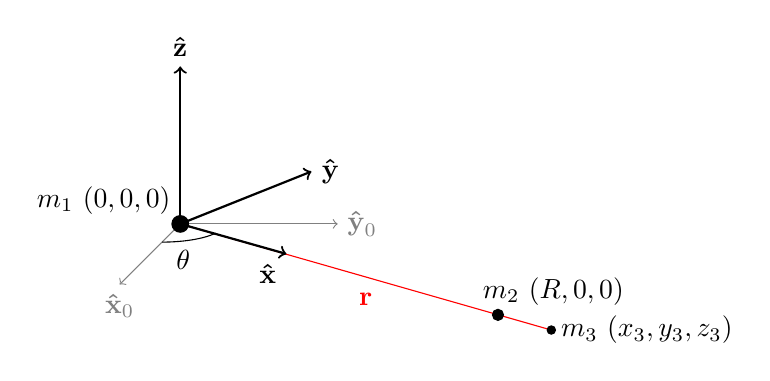
\begin{tikzpicture}
			\coordinate (o) at (0,0,0);
			\draw[thin,gray,->] (0,0,0) -- (0,0,2) node[below] {$\uvec{x}_0$};
			\draw[thin,gray,->] (0,0,0) -- (2,0,0) node[right] {$\uvec{y}_0$};
			
			\draw[red] (o) -- (6.06,0,3.5) node[midway,yshift=-8pt]{$\bvec{r}$};
			
			\draw[thick,->] (0,0,0) -- (0,2,0) node[above] {$\uvec{z}$};
			\draw[thick,->] (0,0,0) -- (1.73,0,0.99) node[below left] {$\uvec{x}$};
			\draw[thick,->] (0,0,0) -- (1,0,-1.73) node[right] {$\uvec{y}$};
			
			\draw (0,0,0.6) arc [start angle=-90,end angle=-32,x radius=0.8,y radius=0.24];
			\node at (.5,0,1.2) {$\theta$};
			
			\filldraw (0,0,0) circle (3pt) node[above left] {$m_1$ $(0,0,0)$};
			\filldraw (5.19,0,3) circle (2pt) node[above,xshift=20pt] {$m_2$ $(R,0,0)$};
			\filldraw (6.06,0,3.5) circle (1.5pt) node[right] {$m_3$ $(x_3,y_3,z_3)$};
		\end{tikzpicture}
	\vspace*{0.25cm}
	\caption{three-dimensional diagram of the Sun-Earth system with unit vectors relative to the Earth's orbit. Not drawn to scale.}
	\label{fig:3d-coords}
	\end{wrapfigure}
	Firstly, we must assert that $m_1 \gg m_2$, meaning that the movement of the Sun due to the gravity of Earth is negligible.
	This allows the Sun to be placed at the center of the coordinate system, avoiding the need to make considerations for the center of mass of the system.
	It is also asserted that $m_2 \gg m_3$, so that, similarly to the previous assertion, the satellite has a negligible effect on Earth.
	Secondly, continuing with the conditions from the previous calculations, it is assumed that the Earth is in a circular orbit, making the system a little easier to comprehend.
	Thirdly, and unlike the previous calculations, we will derive the equations of motion from a inertial reference frame, meaning that we will not be viewing this system from a moving point of reference.
	This will allow us to completely determine motion without the need to consider fictitious forces.
	
	As shown in Figure \ref{fig:3d-coords}, we will have unit vectors $\uvec{x}$, $\uvec{y}$, and $\uvec{z}$ drawn relative to the orbit of the Earth.
	The satellite around L2, $m_3$, will have the coordinates $(x_3,y_3,z_3)$ represented by the vector $\bvec{r}$.
	Taking from my understanding of vectors, the position of a satellite can be expressed as:
	\begin{equation}
		\bvec{r} = x_3\uvec{x} + y_3\uvec{y} + z_3\uvec{z}
	\end{equation}
	Because the unit vectors are not actually static in the system ($\uvec{x}$ and $\uvec{y}$ rotate about the origin), their movement must be taken into account.
	\begin{gather}
		\uvec{x} = (\cos\theta)\uvec{x}_0 + (\sin\theta)\uvec{y}_0 \\
		\uvec{y} = -(\sin\theta)\uvec{x}_0 + (\cos\theta)\uvec{y}_0 \\
		\uvec{z} = \uvec{z}_0
	\end{gather}
	At this point, it is crucial to notice that these equations are not yet useful to us to describe movement.
	In order to describe motion, we need to be able to define the velocity and acceleration of the satellite in three-dimensional space.
	This means being able to take the derivative of a vector.
	Let us assert the following axiom, for some vector \textbf{v} with the basis vectors $\uvec{i}$ and $\uvec{j}$ components $a$ and $b$:
	\begin{equation}
		\frac{d\bvec{v}}{dt} = \frac{da}{dt}\uvec{i} + \frac{db}{dt}\uvec{j}
	\end{equation}
	In other words, the derivative of a vector is the derivative of its components, and would be consistent with the sum rule for derivatives. 
	The notation here can become quite bloated and difficult to read if we continue to use Leibniz's notation.
	So instead, from here on, we will use Newton's notation where possible.
	
	We can take the second derivative of our position vector $\bvec{r}$:
	\begin{equation}
		\bvec{a} = \frac{d^2\bvec{r}}{dt^2} = \frac{d^2x_3\uvec{x}}{dt^2} + \frac{d^2y_3\uvec{y}}{dt^2} + \frac{d^2z_3\uvec{z}}{dt^2}
	\end{equation}
	Our acceleration vector is then expanded to:
	\begin{equation}
		\bvec{a} = \ddot{x}_3\uvec{x} + 2\dot{x}_3\dot{\uvec{x}} + x_3\ddot{\uvec{x}} + \ddot{y}_3\uvec{y} + 2\dot{y}_3\dot{\uvec{y}} + x_3\ddot{\uvec{y}} + \ddot{z}_3\uvec{z} + 2\dot{z}_3\dot{\uvec{z}} + z_3\ddot{\uvec{z}}
	\end{equation}
	
	\section{Plotting the Orbit}
	
	\section{Conclusion}
	
	\newpage
	
	\printbibliography[
	heading=bibintoc,
	title={References}
	]
	
\end{document}